\documentclass[final,hyperref={pdfpagelabels=false}]{beamer}
\usepackage{grffile}
\mode<presentation>{\usetheme{UoL}}
\usepackage[english]{babel}
\usepackage[T1]{fontenc} 
\usepackage[utf8]{inputenc}
\usepackage{amsmath,amsthm, amssymb, latexsym}
\usepackage[scaled=0.98]{helvet}
\usepackage{layouts}
\usepackage{wrapfig}
\usepackage{indentfirst}

\usepackage[caption=false,font=footnotesize]{subfig}
\addto\captionsenglish{\renewcommand{\figurename}{Fig.}}



%\usepackage{times}\usefonttheme{professionalfonts}  % obsolete
%\usefonttheme[onlymath]{serif}
\boldmath
\usepackage[orientation=landscape,size=a0,scale=0.9]{beamerposter}
\usepackage{wrapfig}
\usepackage{comment}
% change list indention level
\setdefaultleftmargin{5em}{}{}{}{}{}
\usepackage[document]{ragged2e}


\usepackage[
backend=biber,
natbib=true,
style=numeric,
sorting=none]{biblatex}
\renewcommand*{\bibfont}{\footnotesize}

\addbibresource{refs.bib}

%\usepackage{snapshot} % will write a .dep file with all dependencies, allows for easy bundling

\usepackage{array,booktabs,tabularx}
\newcolumntype{Z}{>{\centering\arraybackslash}X} % centered tabularx columns
\newcommand{\pphantom}{\textcolor{ta3aluminium}} % phantom introduces a vertical space in p formatted table columns??!!
\usepackage{parcolumns}

\listfiles

%%%%%%%%%%%%%%%%%%%%%%%%%%%%%%%%%%%%%%%%%%%%%%%%%%%%%%%%%%%%%%%%%%%%%%%%%%%%%%%%%%%%%%
\graphicspath{{../../Figures/}{./figures/}}

\title{\huge An Investigation into Physical and Communications Trust Frameworks \\
for Collaborative Teams of Autonomous Underwater Vehicles}
\author{Andrew Bolster, Prof. Alan Marshall, Prof. Jean-Guy Fontaine }
\institute[UoL]{Advanced Networks Research Group, University of Liverpool, UK}
\date[03/07/14]{July 3rd, 2014}

%%%%%%%%%%%%%%%%%%%%%%%%%%%%%%%%%%%%%%%%%%%%%%%%%%%%%%%%%%%%%%%%%%%%%%%%%%%%%%%%%%%%%%


\def\colwidth{0.2\linewidth}

\usecaptiontemplate{
\small
\structure{\insertcaptionname~\insertcaptionnumber:}
\insertcaption
} 
%%%%%%%%%%%%%%%%%%%%%%%%%%%%%%%%%%%%%%%%%%%%%%%%%%%%%%%%%%%%%%%%%%%%%%%%%%%%%%%%%%%%%%
\begin{document}
\begin{frame}[fragile]
	\begin{columns}[T]
		
		\setlength{\parindent}{1em}
		% ---------------------------------------------------------%
		% Set up a column 
		\begin{column}{\colwidth}
			\begin{beamercolorbox}[center,wd=\textwidth]{postercolumn}
				\begin{minipage}[T]{.99\textwidth}  % tweaks the width, makes a new \textwidth
					\parbox[t]{\textwidth}{ % must be some better way to set the the height, width and textwidth simultaneously
						% Since all columns are the same length, it is all nice and tidy.  You have to get the height empirically
						% ---------------------------------------------------------%
						% fill each column with content            
						%%%%%%%%%%%%
						\begin{block}{Project Background and Outputs}
							\begin{itemize}
								\item Attendance at UComms 2012 (Sestri Levante, Italy)
								\item Poster Presentations in 2012 (Kassam, Oxford) and 20.25 (Heathrow, London and Bagneaux, Paris)
								\item Summer Research Placement with DSTL (Software Systems and Dependability for Autonomous Teams)(20.25, PDW)
								\item Paper Presentation to the Association for the Advancement of Artificial Intelligence (AAAI) \cite{Bolster2014}
								\item Technical Report for the UK/US/CAN/AUS/NZ Technical Cooperation Programme \cite{Bolster2014a}
								\item DSTL CDE Collaboration with NPL and Plextek Ltd. on ``Precision Timing and Navigation, Resilient Time and Location Estimation for Networked Assets'' (CDE 33135)
							\end{itemize}
						\end{block}
												
						%%%%%%%%%%%%
						\begin{block}{Introduction}
							\textbf{Aim of project}: To combine physical and communications observations to assess and maintain trust within mobile, marine, ad-hoc networks
														
														 
							\vspace{0.25\baselineskip}
							Small fleets of AUVs (\textbf{Autonomous Underwater Vehicles}) will be expected to operate in isolated environment, requiring an auditible sense of trust within the remote intra-fleet communications networks, incorporating
														
							\begin{columns}[T]
								\begin{column}{0.416\textwidth}
									
									\begin{itemize}
										\item Communications Activity
										\item Mission Suitability/Capability
										\item Behavioural Monitoring
									\end{itemize}
									
									The use of centrally coordinated trust models presents a single point of failure, and secure communication in marine environments is expensive and time consuming. 
									
								\end{column}
								\begin{column}{0.416\textwidth}
									\begin{figure}[h]
										\centering
										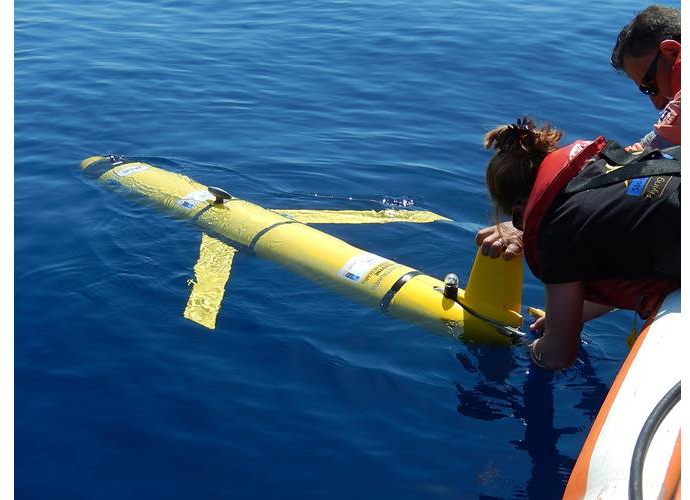
\includegraphics[width=0.8\linewidth]{remus100cmre}
										\vspace{1ex}
										\caption{REMUS 100 AUV, as deployed at CMRE, a potential target platform for this work}
									\end{figure}
								\end{column}
							\end{columns}
							\vspace{0.25\baselineskip}
							Adopting a decentralised form of trust assurance will reduce these costs by localising the per-node security environment.
						\end{block}
						%%%%%%%%%%%%
						\begin{block}{Trust \& Trust Management Frameworks (TMFs)}
							Trust is the expectation of an actor performing a certain task or range of tasks within a certain confidence or probability
														
							Individual trust opinions are shared within the network concerning a range of activities:
							\begin{itemize}
								\item Transmission Routing (Local and/or Back-haul)
								\item Position Reporting
								\item Reporting Accuracy
							\end{itemize}
							\vspace{0.25\baselineskip}
														
							These Trust opinions also apply to extra-fleet entities, such as surface platforms, submarine comms. links, and coastal stations, allowing the fleet to collaboratively form an opinion of these actors.
							
							TMFs are protocols designed to provide information regarding the estimated future states and operations of nodes within networks
							\vspace{0.25\baselineskip}
														
							``[\ldots]collecting the information necessary to establish a trust relationship and dynamically monitoring and adjusting the existing trust relationship'' - \cite{Li2007}
														
							\begin{columns}[T]
								\begin{column}{0.416\textwidth}
									Enables nodes to form collaborative \textbf{opinions} on their cohort nodes based on
									\begin{itemize}
										\item Direct Observation of Behaviour
										\item Common-Neighbour Recommendation
										\item Indirect Reputation
									\end{itemize}
								\end{column}
								\begin{column}{0.416\textwidth}
									\begin{figure}[H]
										\centering
										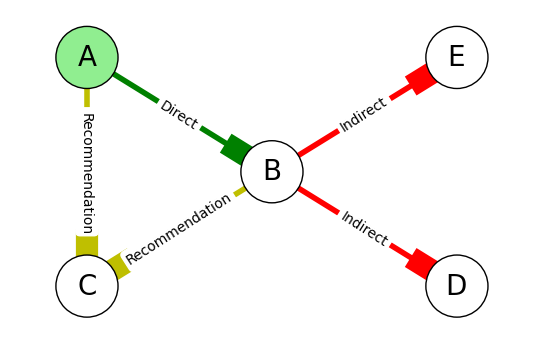
\includegraphics[width=\linewidth]{node_relationships}
										\vspace{1ex}
										\caption{Direct, Recommendation, \& Indirect trust relationships}
									\end{figure}
								\end{column}
							\end{columns}
														
							\vspace{0.25\baselineskip}
														
							Multiple transitive relationships can be maintained over time, providing trust resilience with dynamic network topologies 
														
						\end{block}
						%%%%%%%%%%%%
					}
				\end{minipage}
			\end{beamercolorbox}
		\end{column}
		% ---------------------------------------------------------%
		% end the column
				
		% ---------------------------------------------------------%
		% Set up a column 
		\begin{column}{\colwidth}
			\begin{beamercolorbox}[center,wd=\textwidth]{postercolumn}
				\begin{minipage}[T]{.98\textwidth} % tweaks the width, makes a new \textwidth
					\parbox[t]{\textwidth}{ % must be some better way to set the the height, width and textwidth simultaneously
						% Since all columns are the same length, it is all nice and tidy.  You have to get the height empirically
						% ---------------------------------------------------------%
						% fill each column with content
						%%%%%%%%%%%%
						
						\begin{block}{The Need for Multi-Domain Trust in Autonomous Systems}
							Communications not the only target for an attacker (or failure);
							\begin{itemize}
								\item Following to restricted area
								\item Masquerading
								\item Hardware Degradation
								\item Resource attack
							\end{itemize}
							
							Potential attacks exist within a multi-domain threat surface, and as further metrics and domains of trust are included in a TMF, attackers are increasingly restricted in their behaviour until the only way to avoid detection is to behave correctly.
							\begin{figure}[h]
								\centering
								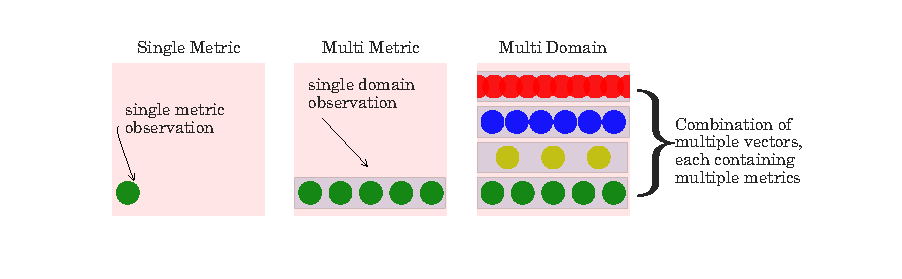
\includegraphics[width=0.9\linewidth]{threat_surface_sum}
								\caption{Threat Surface for Trust Management Frameworks}
							\end{figure}
						\end{block}
												
												
						%%%%%%%%%%%%
						\begin{block}{Multi-Metric Trust Assessment}
							Most TMFs can be generalised as single-metric estimators based on a binary input stats (Packet Loss/Delivery Rates), which provides malicious actors advantage if their activity does not affect that metric. MTFM\cite{Guo11} analyses more than PLR to make it's assessment, including Received and Transmitted signal strength, delay, and throughput as well as taking account of dynamic network topology to inform assessment.
							
							\begin{align}
								\label{eq:grc}
								[\theta_{k,j}^t,\phi_{k,j}^t] & = \frac{\min_k|a_{k,j}^t - r_j^t| + \rho \max_k|a_{k,j}^t-r_j^t|}{|a_{k,j}^t-r_j^t| + \rho \max_k|a_{k,j}^t-r_j^t|},  r \in [g,b] \\
								\label{eq:metric_weighting}
								[\theta_k^t, \phi_k^t]        & = \left[\sum_{j=0}^M h_j \theta_{k,j}^t,\sum_{j=0}^M h_j \phi_{k,j}^t \right]                                                     \\
								\label{eq:trust_value}
								T_k^t                         & = ({1+{(\phi_k^t)^2}/{(\theta_k^t)^2}})^{-1}                                                                                      
							\end{align}
							where $a_{k,j}^t$ is the value of an observed metric $x_j$ for a given node $k$ at time $t$, $\rho$ is a distinguishing coefficient set to $0.5$, $g$ and $b$ are respectively the ``good'' and ``bad'' reference metric sequences from $a$, i.e. $g_j=\max_k({a_{k,j}^t})$,  $b_j=\min_k({a_{k,j}^t})$ 
							
							These metric coefficients are then accumulated \eqref{eq:metric_weighting} and combined to present a singular trust value for analysis \eqref{eq:trust_value}.
							
							
						\end{block}
						%%%%%%%%%%%%
						\begin{block}{Operational Mission Profiles}
							Generic mobility behaviours currently under investigation include:
							\begin{itemize}
								\item \textbf{Waypointing} - Pre-described patrol routes
								\item \textbf{Surveying} - Persistent coverage of an area.
								\item \textbf{Dynamic Constraint} - Repulsion from points (geofencing).
							\end{itemize}
														
							Potentially Exploitable Behaviours not yet developed include:
							\begin{itemize}
								\item \textbf{Capacity Based Homing} - e.g. periodic refuelling
								\item \textbf{Dynamic Communications} - Adjust to changing backhaul
							\end{itemize}
							
							A series of 'Malicious' and 'Faulty' misbehaviours have been designed:
							\begin{itemize}
								\item \textbf{Shadow} - Following the fleet without restricted mission data
								\item \textbf{Spy} - A node that intermittently rises in the fleet, potentially surfacing to relay mission information to a third party
								\item \textbf{Sloth} - Selfish energy conservation by taking minimal paths
								\item \textbf{Stalker} - Tailing a specific node, attempting to use this consistent history to poison the trust network
								\item \textbf{Scoundrel} - Falsely reporting its estimated position with the intention to corrupt collaborative localisation or induce a collision
								\item \textbf{Slow Coach} - Where a node's power train is damaged, causing reduced manoeuvrability and performance
								\item \textbf{Spin Doctor} - Damage to control surfaces or to Inertial Navigation System
							\end{itemize}
							
						\end{block}
												
												
					}
				\end{minipage}
			\end{beamercolorbox}
		\end{column}
		% ---------------------------------------------------------%
		% end the column
				
		% ---------------------------------------------------------%
		% Set up a column 
		\begin{column}{\colwidth}
			\begin{beamercolorbox}[center,wd=\textwidth]{postercolumn}
				\begin{minipage}[T]{.98\textwidth} % tweaks the width, makes a new \textwidth
					\parbox[t]{\textwidth}{ % must be some better way to set the the height, width and textwidth simultaneously
						%%%%%%%%%%%%
						\begin{block}{Behavioural Analysis}
							Three fleets are simulated performing a simple 8 hour patrol mission. The first included a malicious node attempting to infiltrate the fleet (Shadow). The second has a faulty but otherwise "good" node (SlowCoach). The third is a baseline fleet with all "good" nodes
														
							\vspace{0.25\baselineskip}
														
							Physical Metrics under assessment:
							\begin{itemize}
								\item \textbf{INHD}: Inter Node Heading Deviation, or the per-node variation from the fleet-average direction
								\item \textbf{Node Speed}: The Magnitude of Velocity of each node compared to the fleet-average
								\item \textbf{INDD}: Inter Node Distance Deviation, or the variation between the inter-node distances between each node
							\end{itemize}
														
							\begin{figure}
								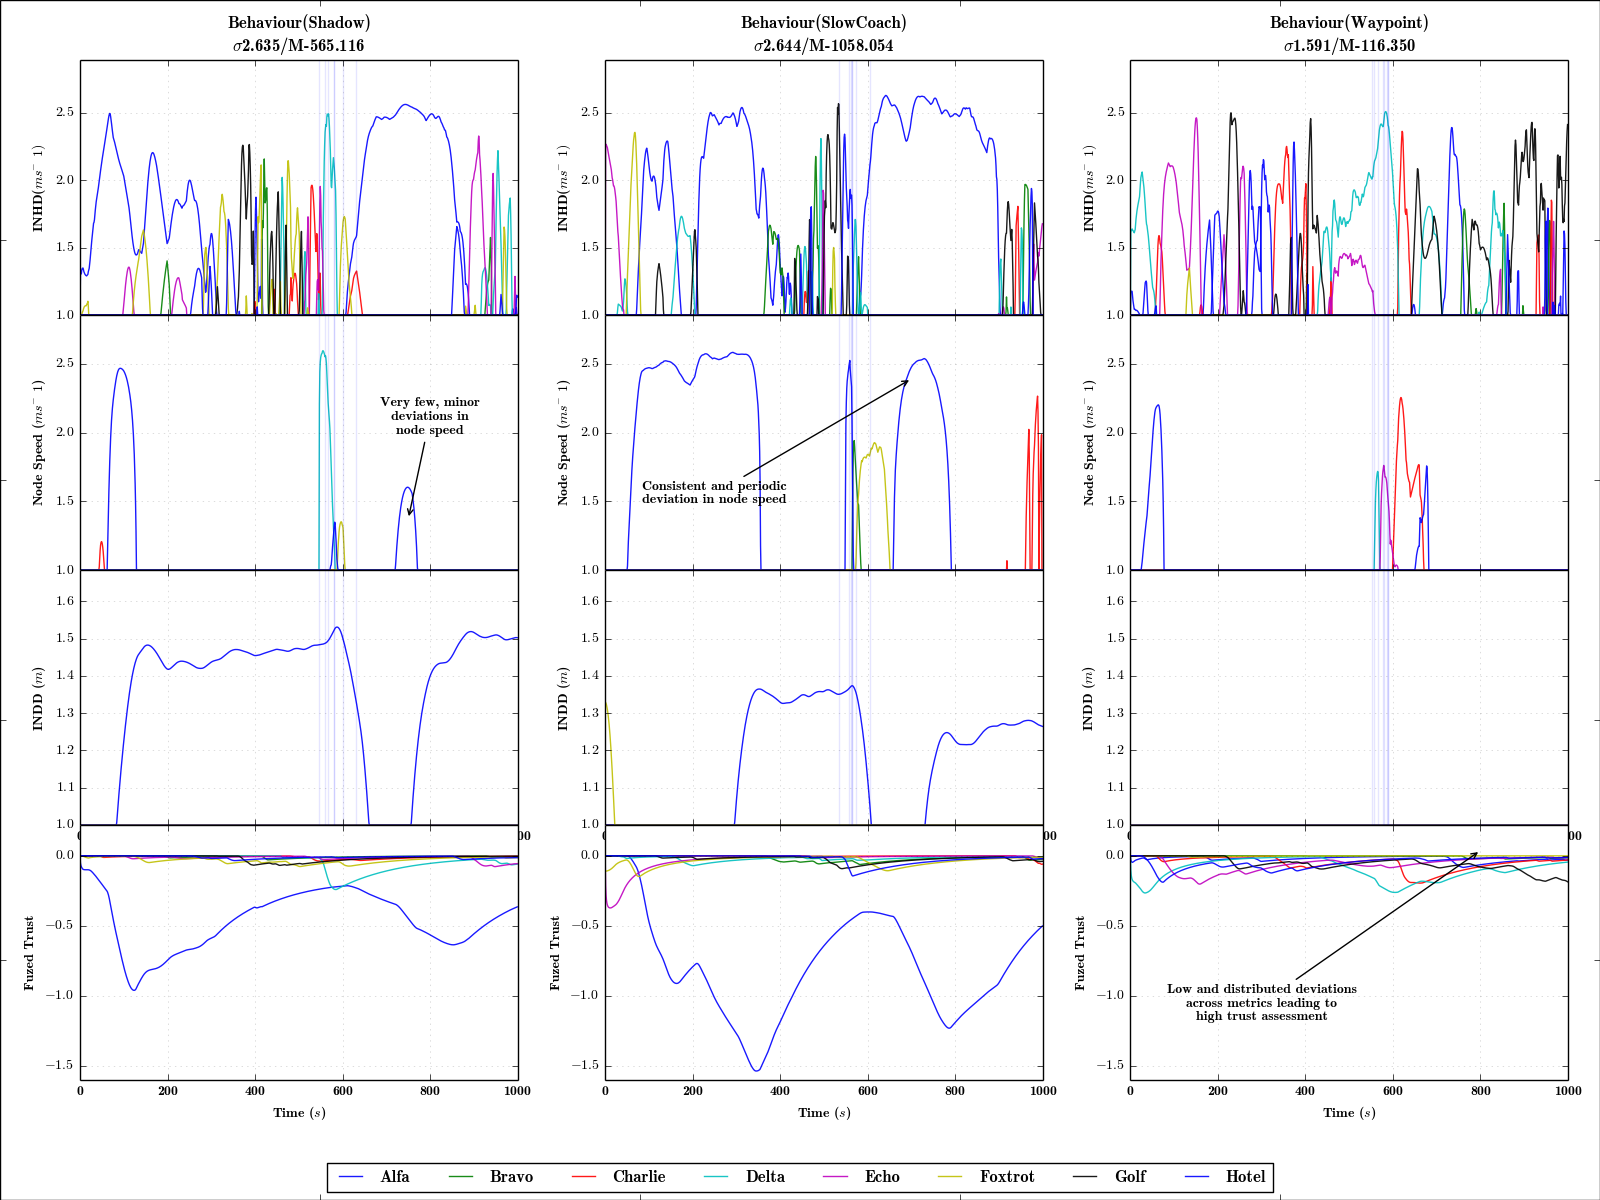
\includegraphics[width=0.95\textwidth]{figures/Bad_Alfa_Fusion}
								\caption{Per-Node deviations for each metric, with an additional row showing an EWMA based cross-metric trust assessment }
								\label{fig:Bad_Alfa_Fusion}
							\end{figure}
														
							From Fig. ~\ref{fig:Bad_Alfa_Fusion}, \textbf{INDD} is a clear candidate for a suspicion 'trigger', but looking at \textbf{INHD} values after several minutes of mission time; an anomaly is clearly being detected. 
														
							\vspace{0.25\baselineskip}
														
							In addition, \textbf{Alfa} node (Blue) is clearly an outlier in terms of \textbf{INHD} and \textbf{Node Speed} in the earliest sections of the graph, and this is shown in the Fused Trust results, however the difference in expression in Node Speed enables not only detection but classification of misbehaviour with a high degree of selectivity (97\%).
														
						\end{block}
						
						%%%%%%%%%%%%
						\begin{block}{Single and Multi-Metric TMF operation in Marine Comms.}
							Acoustic Network based on AUVNetSim \cite{Miquel2008} and validated against \cite{Stefanov2011}.
							
							\vspace{0.25\baselineskip}
														
							Aim to investigate use of Multi-Parameter Trust Framework for MANETS (MTFM), against current communications TMFs (Hermes/ OTMF), which exclusively use Packet Loss Rate (PLR) as their assessment metric.  
							
							\vspace{0.25\baselineskip}
														
							Two Communications Misbehaviours were created: \textbf{Malicious Power Control}(MPC) where a malicious node ($n_1$) inflates it's power to all nodes except a target node ($n_0$) making it appear selfish and \textbf{Selfish Target Selection}(STS) where $n_1$ preferentially communicates with nodes that are physically near-by, reducing its own power consumption.
							
							\begin{figure}[t]
								\subfloat[Fair Scenario]{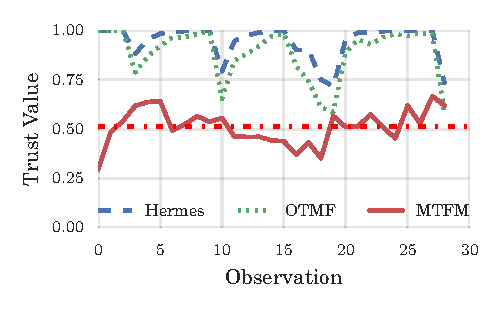
\includegraphics[width=.33\linewidth]{trust_beta_otmf_fair} \label{fig:all_mobile_fair_beta}}
								\subfloat[MPC Scenario]{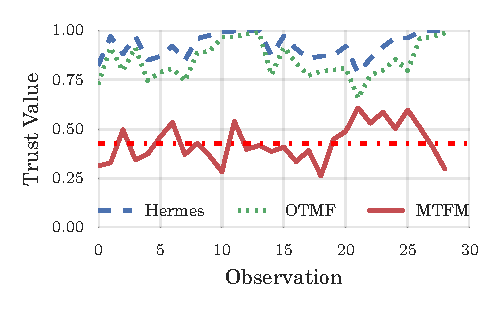
\includegraphics[width=.33\linewidth]{trust_beta_otmf_malicious} \label{fig:all_mobile_badmouthing_beta}}
								\subfloat[STS Scenario]{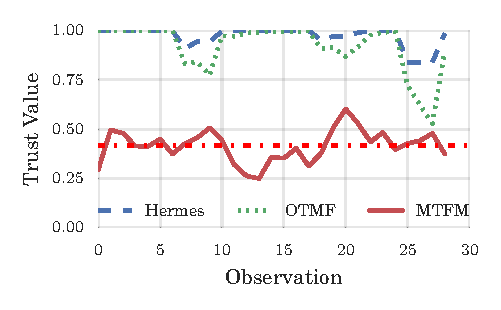
\includegraphics[width=.33\linewidth]{trust_beta_otmf_selfish} \label{fig:all_mobile_selfish_beta}}
								\caption{$T_{1,0}$ for Hermes, OTMF and MTFM assessment values for fair and malicious behaviours in the fully mobile scenario (mean of MTFM also shown)}
								\label{fig:otmf_beta_comparison}
							\end{figure}
							
							From ~\ref{fig:otmf_beta_comparison}, in the challenging underwater environment, no assessment tool is able to appreciably differentiate between behaviours (while MTFM does display a 10\% discriminating behaviour in the a-postori average assessment, shown as a red dashed line)
						\end{block}
						
						%%%%%%%%%%%%


						
					}
					% ---------------------------------------------------------%
					% end the column
				\end{minipage}
			\end{beamercolorbox}
		\end{column}
		% ---------------------------------------------------------%
				
		% ---------------------------------------------------------%
		% Set up a column 
		\begin{column}{\colwidth}
			\begin{beamercolorbox}[center,wd=\textwidth]{postercolumn}
				\begin{minipage}[T]{.98\textwidth} % tweaks the width, makes a new \textwidth
					\parbox[t]{\textwidth}{ % must be some better way to set the the height, width and textwidth simultaneously
						% Since all columns are the same length, it is all nice and tidy.  You have to get the height empirically
						% ---------------------------------------------------------%
						% fill each column with content

						\begin{block}{Metric Permutation and Classification}
							The weights used in \eqref{eq:metric_weighting} can be used to interrogate the trust value space, putting more emphasis on one or more metrics to identify and better characterise a misbehaviour.
							Using this process we can extract and highlight the primary aspects of an attack (MPC/STS) by comparing against the deviation from the ``fair'' result set. 
							
							\begin{figure}[h]
								\centering
								\subfloat[Delay Emphasised]{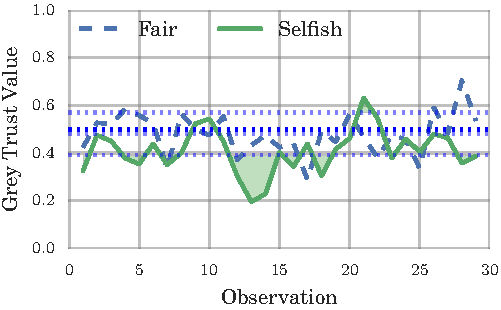
\includegraphics[width=.45\linewidth]{trust_bella_all_mobile_emph_ADelay_SelfishTargetSelection} \label{fig:all_mobile_selfish_delay}}
								\subfloat[PLR Emphasised]{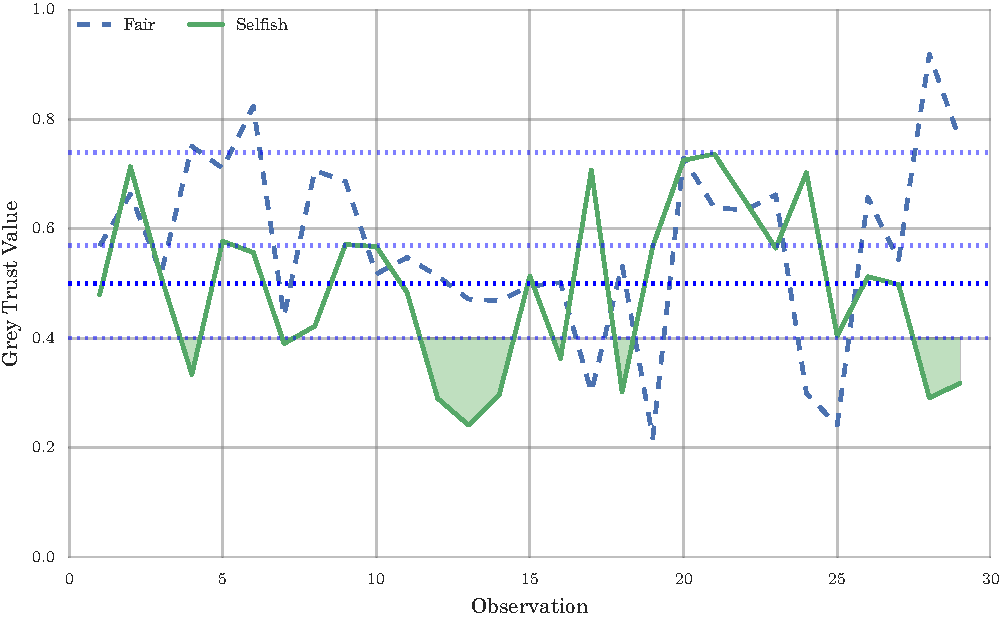
\includegraphics[width=.45\linewidth]{trust_bella_all_mobile_emph_PLR_SelfishTargetSelection}\label{fig:all_mobile_selfish_plr}}
								\newline
								\subfloat[RX Power Emphasised]{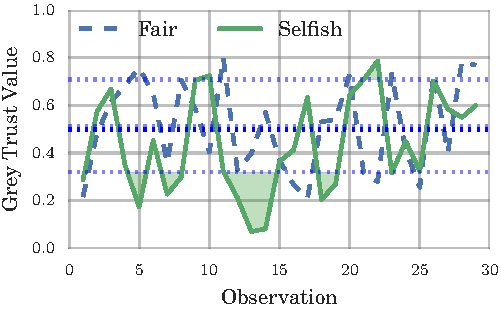
\includegraphics[width=.45\linewidth]{trust_bella_all_mobile_emph_ARXP_SelfishTargetSelection} \label{fig:all_mobile_selfish_rxp}}
								\subfloat[TX Power Emphasised]{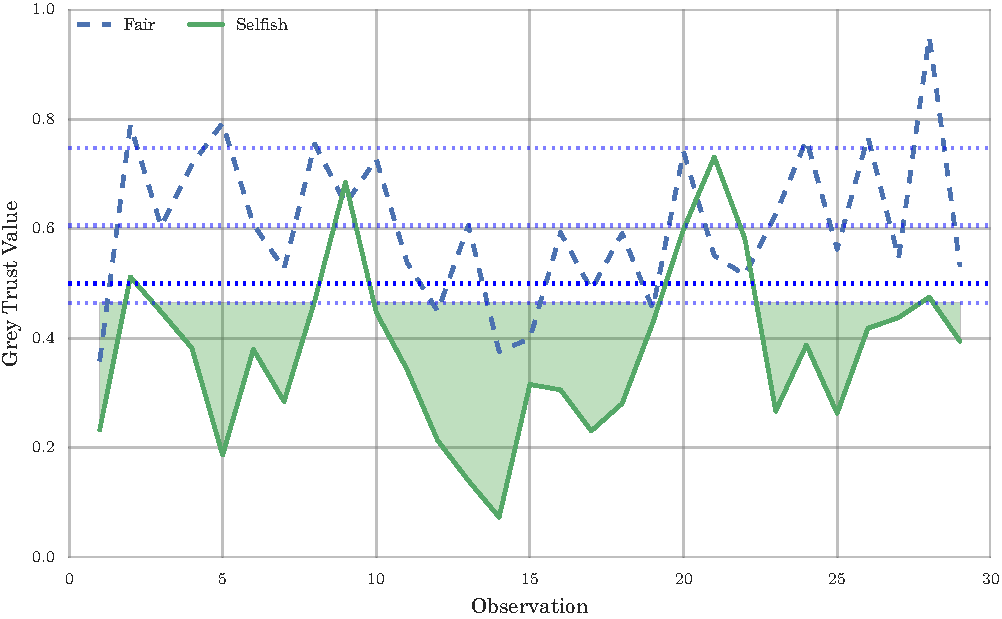
\includegraphics[width=.45\linewidth]{trust_bella_all_mobile_emph_ATXP_SelfishTargetSelection}\label{fig:all_mobile_selfish_txp}}
								\newline
								\subfloat[RX Throughput Emphasised]{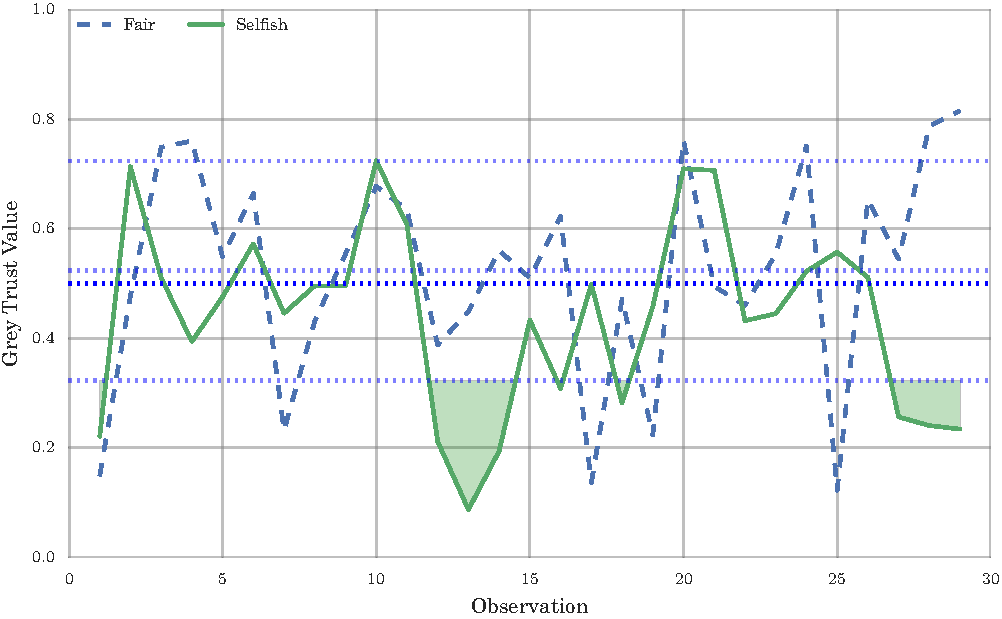
\includegraphics[width=.45\linewidth]{trust_bella_all_mobile_emph_RXThroughput_SelfishTargetSelection} \label{fig:all_mobile_selfish_rxthroughput}}
								\subfloat[TX Throughput Emphasised]{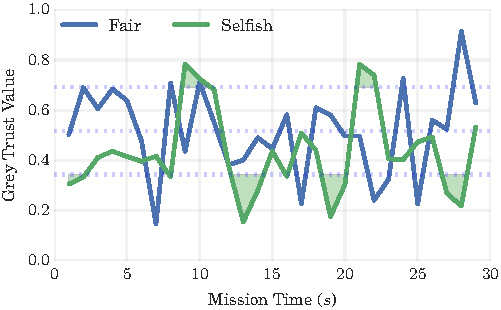
\includegraphics[width=.45\linewidth]{trust_bella_all_mobile_emph_TXThroughput_SelfishTargetSelection} \label{fig:all_mobile_selfish_txthroughput}}
								\caption{$T_{1,MTFM}$ in the All Mobile case for the STS behaviour, including dashed $\pm\sigma$ envelope about the fair scenario}
								\label{fig:all_mobile_selfish}
							\end{figure}
							
						\end{block}						
						%%%%%%%%%%%%
						\begin{block}{Weight Significance Analysis for Behaviour Classification}
							\begin{columns}[T]
								\begin{column}{0.416\textwidth}
								Applying a Random Forest regression tree to 729 different weighting schemes for each of the three behaviours. We assess how important each metric is in differentiating between behaviours; clearly demonstrating that PLR is not an important metric in this regard, where as Received Throughput $T_{RX}^P$ is a major discriminator between STS and MPC.
								\end{column}
								\begin{column}{0.416\textwidth}
								\begin{figure}
									\centering
									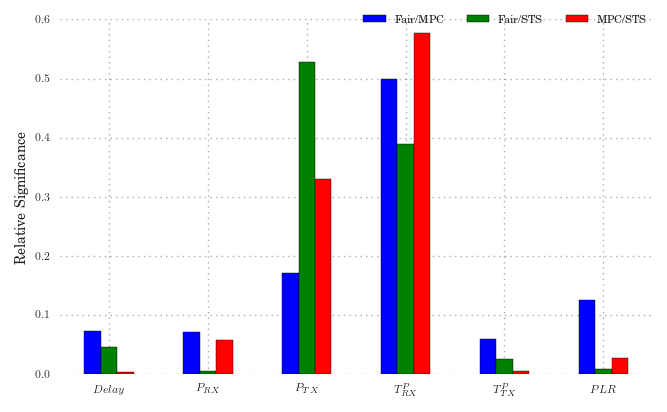
\includegraphics[width=\linewidth]{MaliciousSelfishMetricFactors}
									\caption{Factor Analysis of Malicious (MPC), Selfish (STS) and Fair behaviours selectivity}
									\label{fig:malselfactors}
								\end{figure}
							\end{column}
							\end{columns}
							\begin{table}[h]
								\caption{Correlation Coefficients between metric weights and behaviour detection targets} \label{tab:correlations}
								\begin{center}
									\begin{tabular}{lcccccc}
										\toprule
										Correlation      & Delay & $P_{RX}$ & $P_{TX}$ & $T^P_{RX}$ & $T^P_{TX}$ & PLR \\
										\midrule
										Fair / MPC       & 0.199 &  0.159   & -0.416  &  0.708   & -0.238   & -0.401\\
										Fair / STS       & 0.179 &  -0.009  &  0.724  & -0.697   & -0.145   & -0.052\\
										MPC / STS        & 0.058 &  -0.134  &  0.146  & -0.768   &  0.052   &  0.146\\
										\bottomrule
									\end{tabular}
								\end{center}
							\end{table}
						\end{block}
						%%%%%%%%%%%%
						
						%%%%%%%%%%%%
						\begin{block}{Future Applications}
							\begin{itemize}
								\item Due to the high communications, motion, and computation costs, and lack of external location reporting (\textbf{e.g. GPS}), 
								behavioural analysis in the marine environment is particularly difficult, but if successful, can be reliably applied in a wide 
								variety of fields including but not limited to
								\begin{itemize}
									\item Self-Driving Cars
									\item Environmental Survey drones (terrestrial, marine, and aerial)
									\item Satellite Communications Arrays
									\item Internet Certificate Authority verification
									\item Verifiable Distributed Computing
								\end{itemize}
							\end{itemize}              
						\end{block}
						%%%%%%%%%%%%
												
					}
					% ---------------------------------------------------------%
					% end the column
				\end{minipage}
			\end{beamercolorbox}
		\end{column}
		% ---------------------------------------------------------%
		% end the column   % end the column
		% ---------------------------------------------------------%
		% Set up a column 
		\begin{column}{\colwidth}
			\begin{beamercolorbox}[center,wd=\textwidth]{postercolumn}
				\begin{minipage}[T]{.98\textwidth} % tweaks the width, makes a new \textwidth
					\parbox[t]{\textwidth}{ % must be some better way to set the the height, width and textwidth simultaneously
						% Since all columns are the same length, it is all nice and tidy.  You have to get the height empirically
						% ---------------------------------------------------------%
						% fill each column with content
						%%%%%%%%%%%%
												
						\begin{block}{Conclusions}
							This research area presents a range of challenges and opportunities within both civil and defence operations; an auditable trust framework for automated marine craft would be a significant enabling factor to the roll-out of more low-maintenance or even ``Fire and Forget'' deployments for persistent patrol/monitoring tasks. 
														
							\vspace{0.25\baselineskip}
														
							Open Hypotheses in this field that this project intends to answer are:
							\begin{itemize}
								\item How can optimality in trust assessment based on behaviour be defined win a distributed, dynamic network topology?
								\item Is there a quantifiable benefit to cross-domain comparison beyond single-vector trust? (i.e. 1-D vector vs cross domain comparison)
								\item Is there an optimal \textbf{generic} cross domain fusion methodology?
							\end{itemize}
						\end{block}
						%%%%%%%%%%%%
						\begin{block}{Thesis Plan}
							\begin{itemize} 
								\item Trust and its applications to MANETs
								\begin{itemize}
									\item Discussion on abstract analysis of trust networks
									\item Discussion on the threat surface of Mobile Ad Hoc Networks and how that has been protected so far
									\item Introduction to Trust Management Frameworks and their benefits
								\end{itemize}
								\item Maritime Uses of Autonomous Systems
								\begin{itemize}
									\item Discussion of current and future approaches to areas where autonomous systems can be used mainly focused on Mine counter measures, Hydrography and Patrol Capabilities (MHPC)
									\item Discussion of the contextual human factors around integrating autonomous systems into existing human-based solutions, predominantly following on from \cite{Bolster2014a}, including development of representative malicious and abnormal behaviours
								\end{itemize}
								\item Strategies for Multi-Domain Trust Assessment
								\begin{itemize}
									\item Analytical establishment of Multi-Domain Trust, from an information theoretic standpoint.
								\end{itemize}
								\item Modelling and Analysis of Collaborative Node Kinematic Behaviours in Underwater Acoustic MANETS
								\begin{itemize}
									\item Focused on the mobility and assessment of mobility between nodes, including identification of suitable motive metrics and analyses of these motions to establish intent or abnormality
									\item Incorporating collaboration with NPL/Plextek as supporting evidence.
								\end{itemize}
								\item Comparative Analysis of Multi-Domain Trust Assessment in Collaborative Mobile Networks
								\item Investigation into the relative performance characteristics of multi-domain combination strategies in an exemplary context (AUV teams) against existing single and multi metric TMFs
							\end{itemize}
														
						\end{block}
												
												
						%%%%%%%%%%%%
												
												
						\begin{block}{Bibliography}						
							\printbibliography[title=References]% [nottype=video]}
						\end{block}
					}
					% ---------------------------------------------------------%
					% end the column
				\end{minipage}
			\end{beamercolorbox}
		\end{column}
		% ---------------------------------------------------------%
		% end the column   % end the column
				
	\end{columns}
\end{frame}
\end{document}


%%%%%%%%%%%%%%%%%%%%%%%%%%%%%%%%%%%%%%%%%%%%%%%%%%%%%%%%%%%%%%%%%%%%%%%%%%%%%%%%%%%%%%%%%%%%%%%%%%%%
%%% Local Variables: 
%%% mode: latex
%%% TeX-PDF-mode: t
%%% End:
